\section{Perspective Projection} \label{sec:intrinsics}




Next, we would like to find the intrinsic matrix, $M_{int}$, which relates the positional vector $\vec{p}_c$ of point $P$ in the camera coordinate frame, to its positional vector $\vec{p}_i$ on the image plane. Using $\widetilde{p}_c$ and $\widetilde{p}_i$ to represent the homogenous coordinates of the vectors $\vec{p}_c$ and $\vec{p}_i$ respectively, we can express this mathematically as follows:
\begin{equation} \label{eq:pi}
    \widetilde{p}_i =  M_{ext}\,\widetilde{p}_c
\end{equation}


\begin{figure}[H]
    \centering
    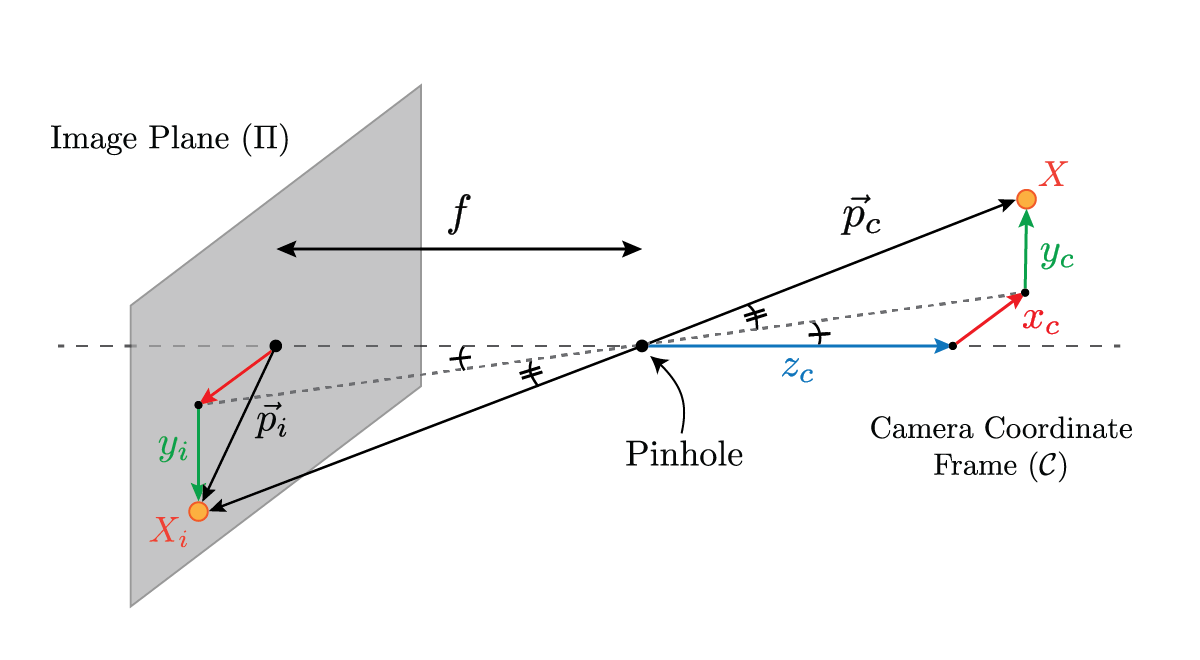
\includegraphics[width=0.9\textwidth]{figures/perspective_projection}
    \caption{Perspective projection of the point onto the image plane $\Pi$.}
\end{figure}

\begin{figure}[H]
    \centering
    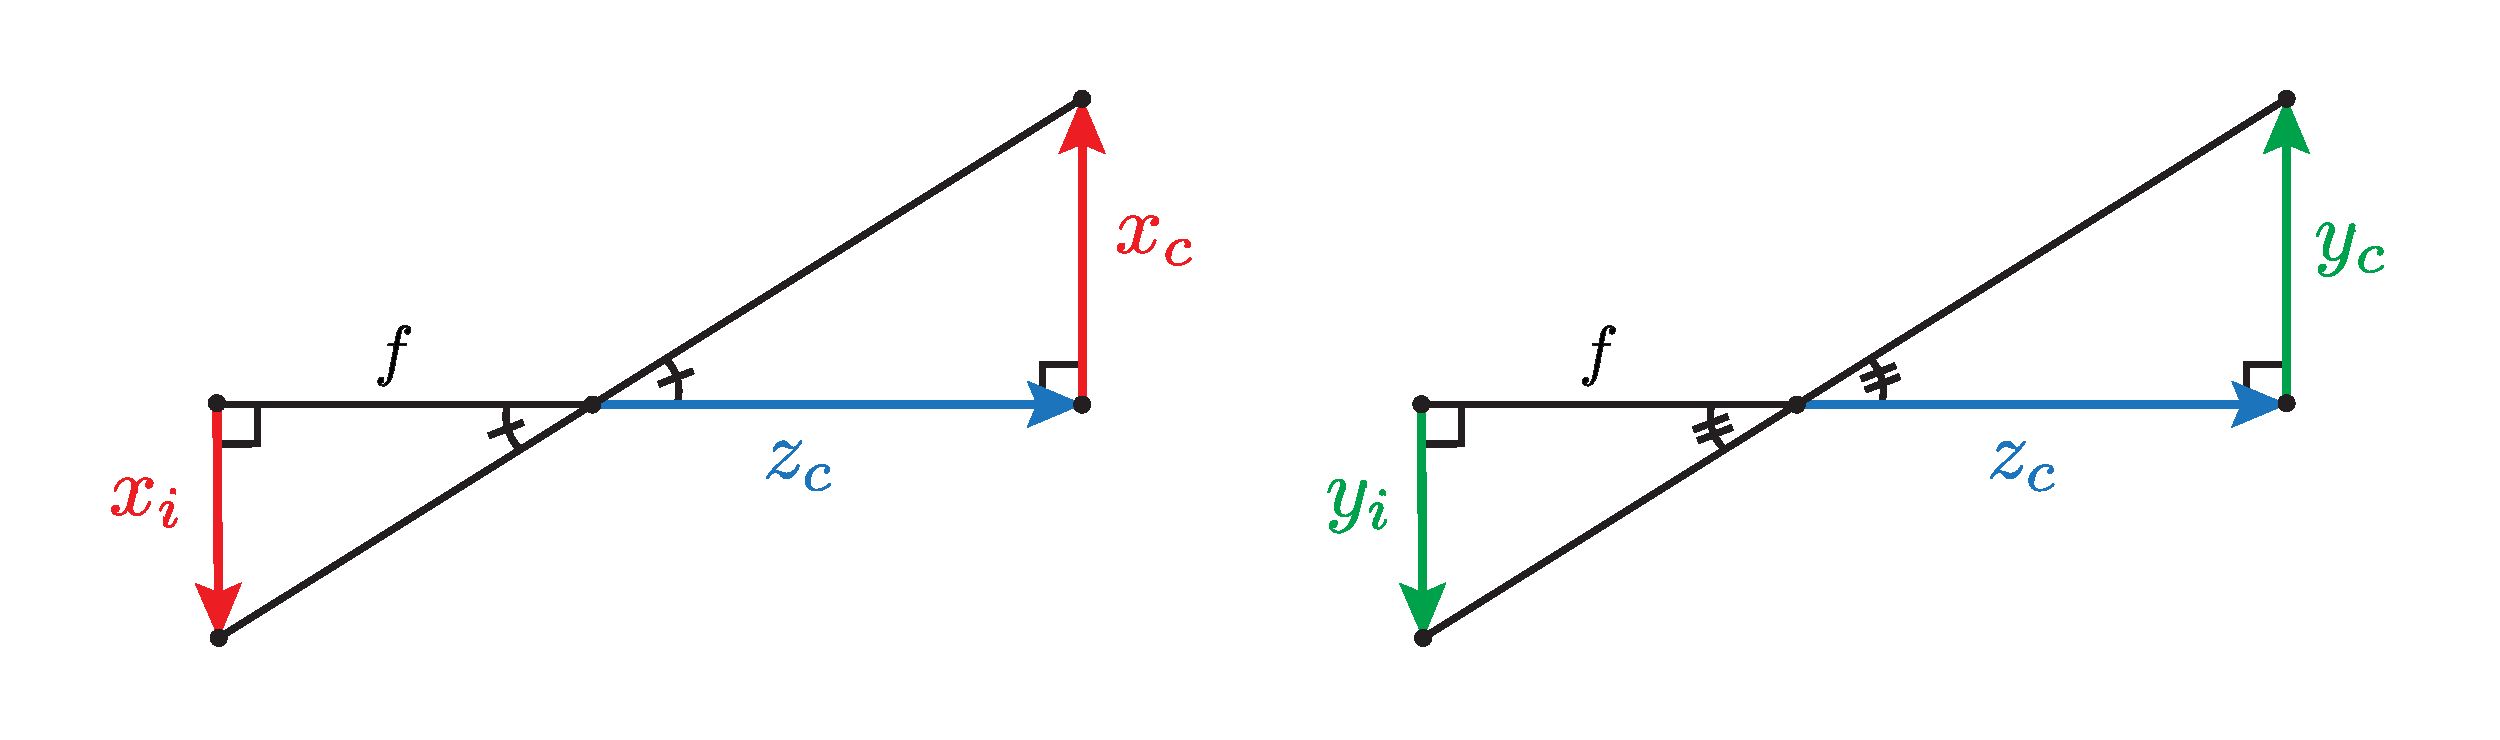
\includegraphics[width=\textwidth]{figures/similar_triangles}
    \caption{Similar triangles formed by perspective projection, which relate $x_i$ to $x_c$ and $y_i$ to $y_c$}
\end{figure}

\begin{subequations}
    \begin{gather}
        \frac{x_i}{f} = \frac{x_c}{z_c} \quad \Longrightarrow \quad x_i = f \frac{x_c}{z_c} \label{subeq:xi_result}\\
        \frac{y_i}{f} = \frac{y_c}{z_c} \quad \Longrightarrow \quad y_i = f \frac{y_c}{z_c} \label{subeq:yi_result}
    \end{gather}
\end{subequations}

We can then relate the coordinates of the projection, $(x_i, y_i)$, which are in real-world units, to its position $(u, v)$ in pixels.
\begin{figure}[H]
    \centering
    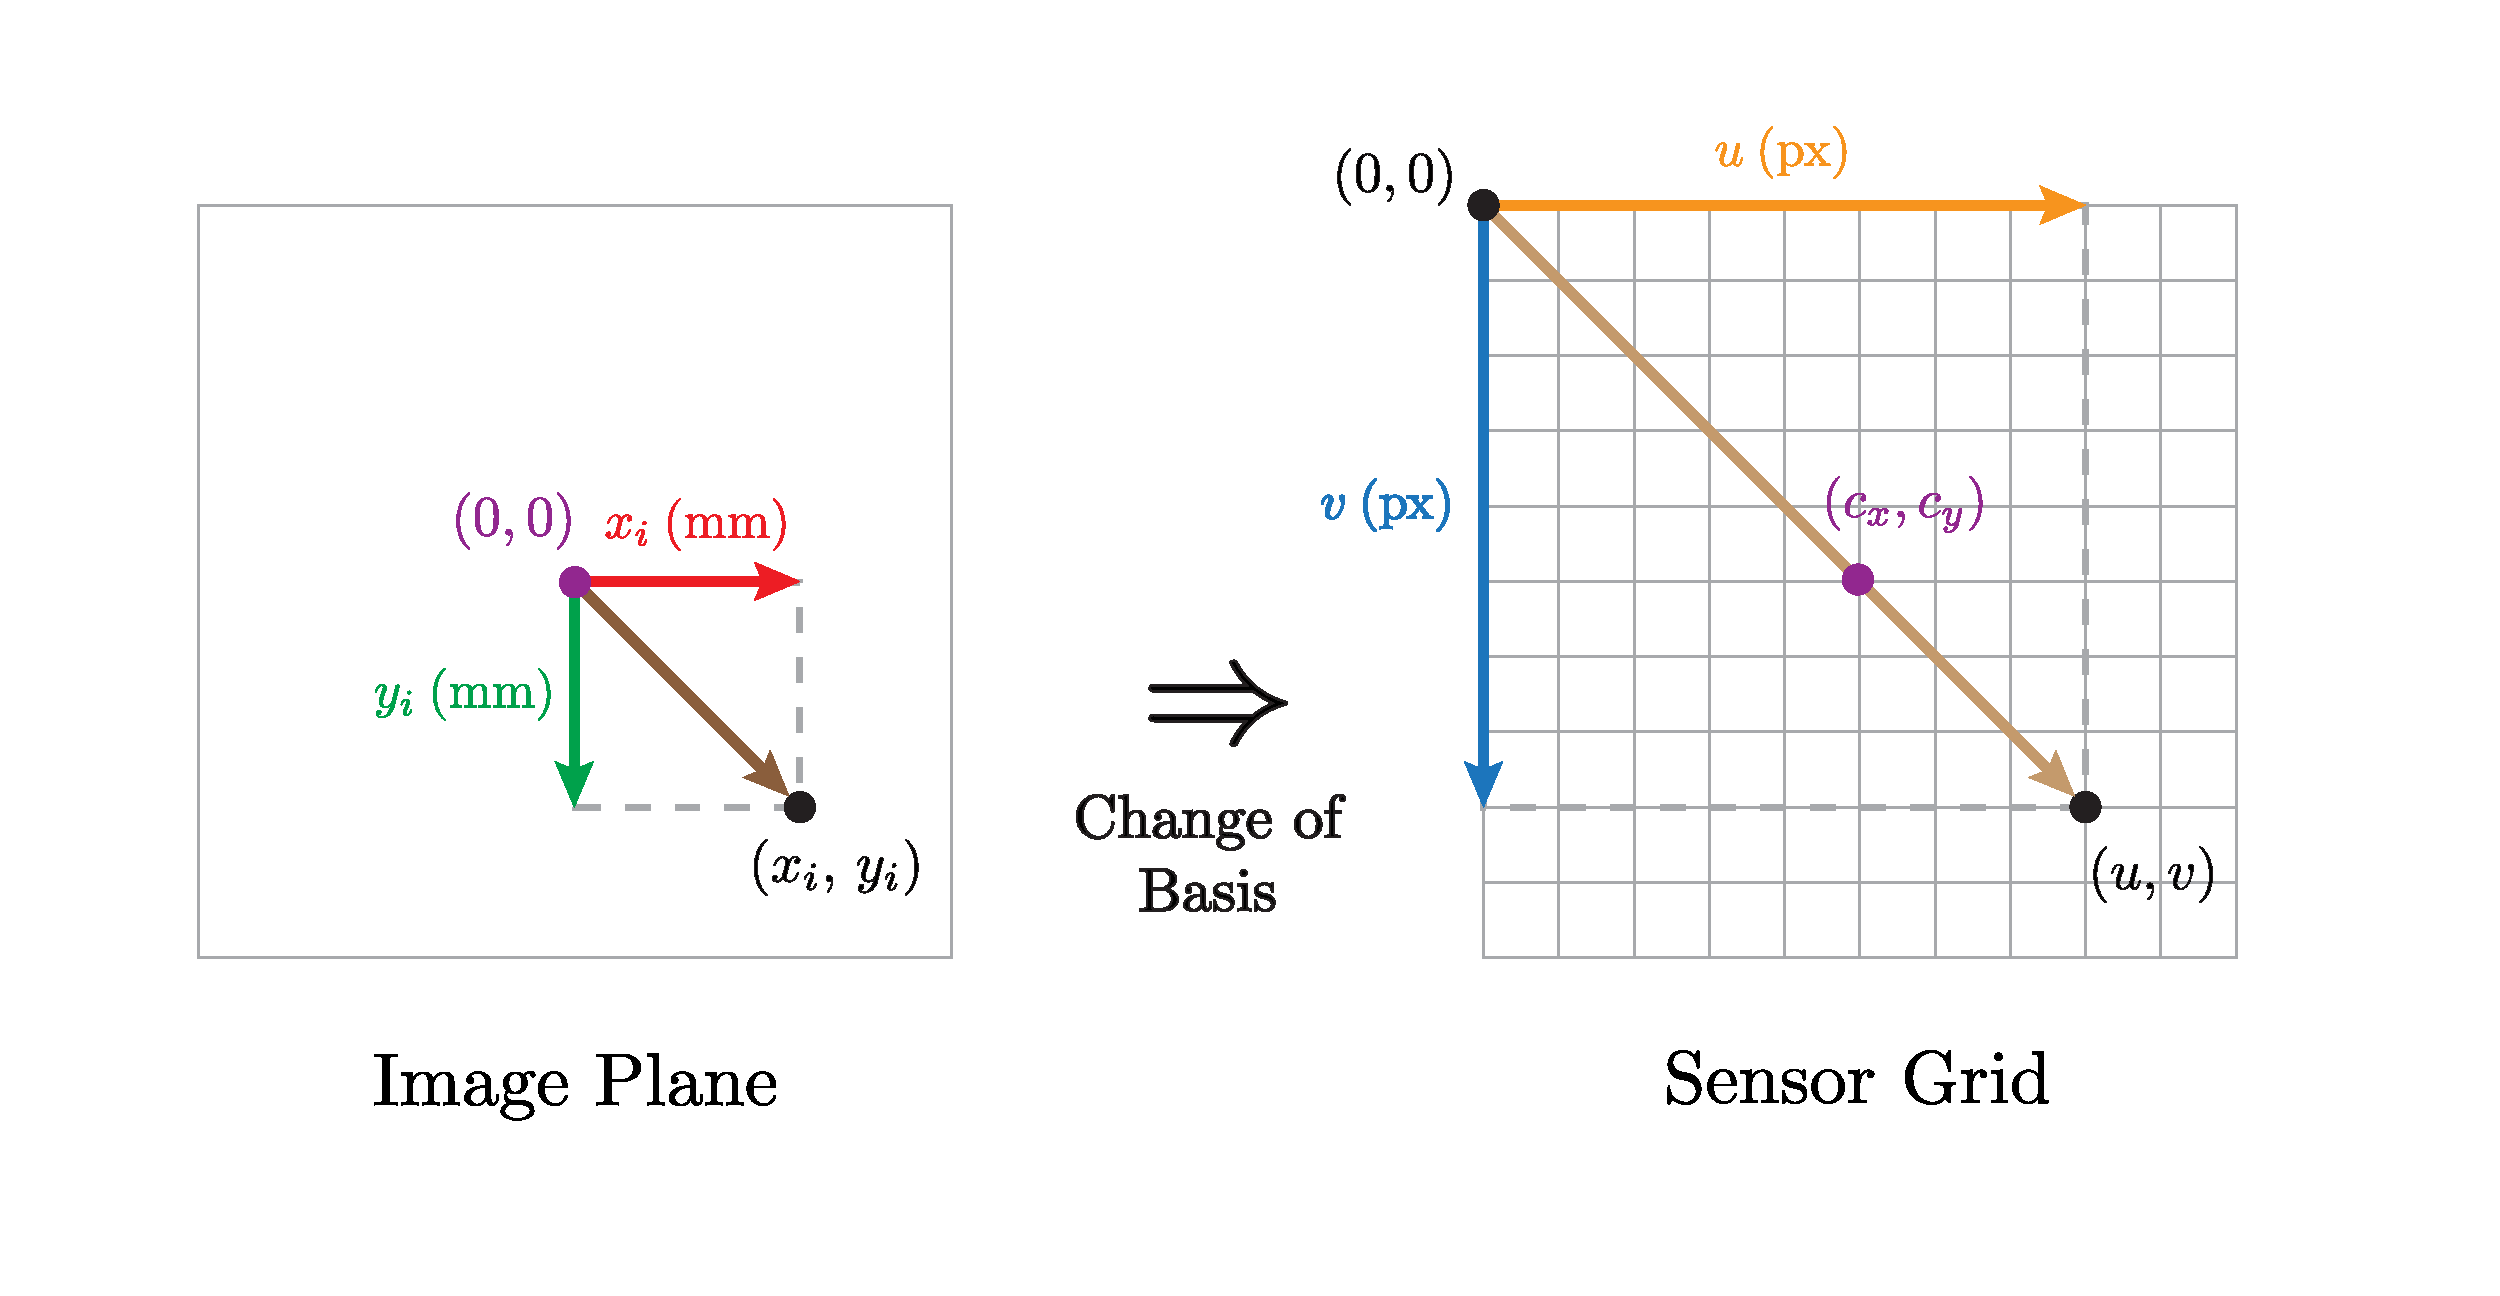
\includegraphics[width=\textwidth]{figures/sensor_grid}
    \caption{Conversion from image plane coordinates to sensor grid coordinates}
\end{figure}
Let $m_x$ and $m_y$ represent the pixel density of the image sensor in the $x$ and $y$ axes of the image sensor plane respectively.
\begin{align*}
    u = m_x x_i + c_x \\
    v = m_y y_i + c_y
\end{align*}
Replacing $x_i$ and $y_i$ for the result we obtained from \ref{subeq:xi_result} and \ref{subeq:yi_result}, we get:
\begin{align*}
    u = m_x f \frac{x_c}{z_c} + c_x \\
    v = m_y f \frac{y_c}{z_c} + c_y
\end{align*}
Since $m_x$, $m_y$, and $f$ are all unknowns, we can combine the products $m_x f$ and $m_y f$ to $f_x$ and $f_y$ respectively. Under this new scheme, we define $f_x$ and $f_y$ as the horizontal and vertical focal lengths of camera.
\begin{subequations}
    \begin{gather}
        u = f_x \frac{x_c}{z_c} + c_x \\
        v = f_y \frac{y_c}{z_c} + c_y
    \end{gather}
\end{subequations}

\subsection{Intrinsic Matrix}

\begin{equation}
    \begin{bmatrix}
        u \\ v
    \end{bmatrix}
    \sim
    \begin{bmatrix}
        \widetilde{u} \\ \widetilde{v} \\ \widetilde{w}
    \end{bmatrix}
    \equiv
    \begin{bmatrix}
        z_c u \\ z_c v \\ z_c
    \end{bmatrix}
    =
    \begin{bmatrix}
        f_x x_c + z_c c_x \\ f_y y_c + z_c c_y \\ z_c
    \end{bmatrix}
    =
    \underbrace{
        \begin{bmatrix}
            f_x & 0   & c_x & 0 \\
            0   & f_y & c_y & 0 \\
            0   & 0   & 1   & 0
        \end{bmatrix}
    }_{\mathlarger{M_{int}}}
    \begin{bmatrix}
        x_c \\ y_c \\ z_c \\ 1
    \end{bmatrix}
\end{equation}


\begin{equation}
    K =
    \begin{bmatrix}
        f_x & 0   & c_x \\
        0   & f_y & c_y \\
        0   & 0   & 1
    \end{bmatrix}
\end{equation}

Note that $K$ that is an \emph{upper triangular matrix}. It is a special kind of square matrix with all of its non-zero entries above the main diagonal. This is an important property which we will exploit when extracting the intrinsic matrix from the projection matrix in section \ref{sec:projection}.

As such, we can express $M_{int}$ as $\left[\: K \:\vert\: 0 \:\right]$.

\begin{equation}
    M_{int} = \left[\: K \:\vert\: 0 \:\right]
\end{equation}
